% Options for packages loaded elsewhere
\PassOptionsToPackage{unicode}{hyperref}
\PassOptionsToPackage{hyphens}{url}
%
\documentclass[
]{article}
\usepackage{amsmath,amssymb}
\usepackage{lmodern}
\usepackage{ifxetex,ifluatex}
\ifnum 0\ifxetex 1\fi\ifluatex 1\fi=0 % if pdftex
  \usepackage[T1]{fontenc}
  \usepackage[utf8]{inputenc}
  \usepackage{textcomp} % provide euro and other symbols
\else % if luatex or xetex
  \usepackage{unicode-math}
  \defaultfontfeatures{Scale=MatchLowercase}
  \defaultfontfeatures[\rmfamily]{Ligatures=TeX,Scale=1}
\fi
% Use upquote if available, for straight quotes in verbatim environments
\IfFileExists{upquote.sty}{\usepackage{upquote}}{}
\IfFileExists{microtype.sty}{% use microtype if available
  \usepackage[]{microtype}
  \UseMicrotypeSet[protrusion]{basicmath} % disable protrusion for tt fonts
}{}
\makeatletter
\@ifundefined{KOMAClassName}{% if non-KOMA class
  \IfFileExists{parskip.sty}{%
    \usepackage{parskip}
  }{% else
    \setlength{\parindent}{0pt}
    \setlength{\parskip}{6pt plus 2pt minus 1pt}}
}{% if KOMA class
  \KOMAoptions{parskip=half}}
\makeatother
\usepackage{xcolor}
\IfFileExists{xurl.sty}{\usepackage{xurl}}{} % add URL line breaks if available
\IfFileExists{bookmark.sty}{\usepackage{bookmark}}{\usepackage{hyperref}}
\hypersetup{
  pdftitle={Large-scale Machine-Learning analysis of scientific PDF to monitor the production and the openness of research data and software in France},
  pdfkeywords={research software, research data, open access, open
science, scientometrics},
  hidelinks,
  pdfcreator={LaTeX via pandoc}}
\urlstyle{same} % disable monospaced font for URLs
\usepackage[left=3cm, right=3cm, top=3cm, bottom=3cm]{geometry}
\usepackage{longtable,booktabs,array}
\usepackage{calc} % for calculating minipage widths
% Correct order of tables after \paragraph or \subparagraph
\usepackage{etoolbox}
\makeatletter
\patchcmd\longtable{\par}{\if@noskipsec\mbox{}\fi\par}{}{}
\makeatother
% Allow footnotes in longtable head/foot
\IfFileExists{footnotehyper.sty}{\usepackage{footnotehyper}}{\usepackage{footnote}}
\makesavenoteenv{longtable}
\usepackage{graphicx}
\makeatletter
\def\maxwidth{\ifdim\Gin@nat@width>\linewidth\linewidth\else\Gin@nat@width\fi}
\def\maxheight{\ifdim\Gin@nat@height>\textheight\textheight\else\Gin@nat@height\fi}
\makeatother
% Scale images if necessary, so that they will not overflow the page
% margins by default, and it is still possible to overwrite the defaults
% using explicit options in \includegraphics[width, height, ...]{}
\setkeys{Gin}{width=\maxwidth,height=\maxheight,keepaspectratio}
% Set default figure placement to htbp
\makeatletter
\def\fps@figure{htbp}
\makeatother
\setlength{\emergencystretch}{3em} % prevent overfull lines
\providecommand{\tightlist}{%
  \setlength{\itemsep}{0pt}\setlength{\parskip}{0pt}}
\setcounter{secnumdepth}{-\maxdimen} % remove section numbering
\ifluatex
  \usepackage{selnolig}  % disable illegal ligatures
\fi
\newlength{\cslhangindent}
\setlength{\cslhangindent}{1.5em}
\newlength{\csllabelwidth}
\setlength{\csllabelwidth}{3em}
\newenvironment{CSLReferences}[2] % #1 hanging-ident, #2 entry spacing
 {% don't indent paragraphs
  \setlength{\parindent}{0pt}
  % turn on hanging indent if param 1 is 1
  \ifodd #1 \everypar{\setlength{\hangindent}{\cslhangindent}}\ignorespaces\fi
  % set entry spacing
  \ifnum #2 > 0
  \setlength{\parskip}{#2\baselineskip}
  \fi
 }%
 {}
\usepackage{calc}
\newcommand{\CSLBlock}[1]{#1\hfill\break}
\newcommand{\CSLLeftMargin}[1]{\parbox[t]{\csllabelwidth}{#1}}
\newcommand{\CSLRightInline}[1]{\parbox[t]{\linewidth - \csllabelwidth}{#1}\break}
\newcommand{\CSLIndent}[1]{\hspace{\cslhangindent}#1}
% for compatibility with pandoc 2.10
\newenvironment{cslreferences}%
  {}%
  {\par}

\title{Large-scale Machine-Learning analysis of scientific PDF to
monitor the production and the openness of research data and software in
France}
\usepackage{etoolbox}
\makeatletter
\providecommand{\subtitle}[1]{% add subtitle to \maketitle
  \apptocmd{\@title}{\par {\large #1 \par}}{}{}
}
\makeatother
\subtitle{Widening the French Open Science Monitor scope}
\usepackage{authblk}
\author[%
  2%
  ]{%
  Aricia Bassinet%
  %
  %
}
\author[%
  2%
  ]{%
  Laetitia Bracco%
  %
  %
}
\author[%
  1%
  ]{%
  Anne L'Hôte%
  %
  %
}
\author[%
  1%
  ]{%
  Eric Jeangirard%
  %
  %
}
\author[%
  3%
  ]{%
  Patrice Lopez%
  %
  %
}
\author[%
  4%
  ]{%
  Laurent Romary%
  %
  %
}
\affil[1]{French Ministry of Higher Education, Research, Paris, France}
\affil[2]{University of Lorraine, France}
\affil[3]{science-miner, France}
\affil[4]{Inria, France}
\date{January 2023}

\makeatletter
\def\@maketitle{%
  \newpage \null \vskip 2em
  \begin {center}%
    \let \footnote \thanks
         {\LARGE \@title \par}%
         \vskip 1.5em%
                {\large \lineskip .5em%
                  \begin {tabular}[t]{c}%
                    \@author
                  \end {tabular}\par}%
                                                \vskip 1em{\large \@date}%
  \end {center}%
  \par
  \vskip 1.5em}
\makeatother

\begin{document}
\maketitle
\begin{abstract}
There is today no standard way for referencing research datasets and
research software in scientific communication. Emerging editorial
workflows and supporting infrastructures dedicated to dataset and
software are still poorly adopted by current publishing practices and
are highly fragmented.

To better follow the production of research datasets and software, we
present a text mining method applied to scientific publications at scale
and implemented at the French national level. Our approach relies on
state-of-the-art Machine Learning and document engineering techniques to
ensure satisfactory accuracy across multiple research areas and document
types, combining full-text harvesting, mention extraction, context
characterization and corpus-level analysis.

The annotations produced by our system are used by the French Open
Science Monitor (BSO)
\href{https://frenchopensciencemonitor.esr.gouv.fr}{platform} to follow
the production and the openness of research data and software, in the
context of the second National Plan for Open Science.

The source code and the data of the French Open Science Monitor, as well
as all the associated tools and datasets, are available under open
licences.
\end{abstract}

\textbf{Keywords}: research software, research data, open access, open
science, scientometrics

\hypertarget{introduction}{%
\section{1. Introduction}\label{introduction}}

\hypertarget{motivations}{%
\subsection{Motivations}\label{motivations}}

Datasets and software are today a core element of the research
activities, whose increasing role is broadly acknowledged {[}{]}. With
the objective of better supporting the reuse and the reproducibility of
research results, many initiatives to improve the visibility of research
dataset and software took place in the last decade, in particular
focusing on improving dataset and software cataloging {[}{]} and
standards for citation {[}{]}.

However, the usage, creation, and sharing information for the large
majority of research data and software are only available in narative
forms inside the content of scientific publications\ldots{} Among the
main reasons, we can mention the lack of incentive for researchers to
invest time on work not credited and not considered for career and
promotion, the fragmentation of policies, standards, infrastructures and
workflows, and the absence of investment by most of the scientific
publishers to implement standard for referencing of dataset and
software.

To address these pitfalls, and as a way to enforce higer standards of
openness and visibility for all research results, national Open Science
policies are currently rapidly developing\ldots{} To measure the effect
of these policies and adapt them to maximize their adoption, monitoring
tool and dashboards are crucial\ldots{}

\hypertarget{the-french-open-science-monitor}{%
\subsection{The French Open Science
Monitor}\label{the-french-open-science-monitor}}

The French Open Science Monitor, also called BSO for `Baromètre de la
Science Ouverte', is a tool for monitoring and steering the public
policy linked to the first French National Plan for Open Science
{[}4{]}. A first version of the tool was launched in 2019 providing
measurements of the rate of Open Access publications produced by all
public French research entities. A follow-up second Plan for Open
Science {[}3{]} has started to further promote and develop the French
open science policy, including a focus on research data and research
software. The French Open Science Monitor is updated every year {[}1{]},
however measurements related to research datasets and software were not
covered yet.

The extension of the French Open Science Monitor to research datasets
and software was funded following a call for projects within the
framework of the French Recovery Plan. The University of Lorraine has
been asked by the Ministry of Higher Education and Research (MESR) to
lead this project alongside the MESR's Department of Decision Support
Tools and Inria.

\hypertarget{quality-criteria-for-open-science-indicators}{%
\subsection{Quality criteria for Open Science
indicators}\label{quality-criteria-for-open-science-indicators}}

What are the quality criteria for useful and reliable indicators on the
production of research datasets and research software ?

\begin{itemize}
\item
  coverage
\item
  accuracy
\item
  freshness
\item
  adaptibility to different geographical and organizational levels
\item
  adaptibility to different scientific and technical domains
\item
  fair: maintain consistency in term of domains and languages
\end{itemize}

Why the current Open Science monitors related to data and software fail
regarding these criteria? e.g.~OpenAire. Extremely limited coverage
leads to extremely biased and unreliable indicators, leading to
counter-productive dashboards (for instance indicating that a handful of
datasets is produced at the scale of a whole University during one
year). Publishing aggregated dashboard on unreliable and
non-representative data can lead to disengagement of the public for the
tool, false interpretation, wrong public policy decisions and unability
to assess public the application of Open Science policies.

Why do we think an automatic data-centric approach to capture the actual
scientific activity and production could lead to higher quality
indicators than the manually referencing approach? Because it can offer
a more trustful snapshot of the scientific production, but it needs to
be reliable enough (precision and coverage) and applied to a very
significant amount of scientific publications.

\hypertarget{challenges}{%
\subsection{Challenges}\label{challenges}}

In view of the slow adoption of more comprehensive formal and manual
reference workflows, mining dataset and software mentions in scientific
publications appeared early as a possible solution to increase at scale
the visibility of these new key research products.

Description of prior works\ldots{} dictionary/term search, regular
expressions, domain-specific rules, restriction to XML full texts
availability. Lack of annotated data and reliable evaluations.

Characterizing the data and software usage and sharing: Often too much
``publication centric'' (e.g.~is the publication uses/shares some data
and code? versus what are the data/code product and how these data and
software are they shared and reused?)

Lack of quality metadata and considerable fragmentation of source code
repositories.

Which indicators should be selected to provide meaningful information on
data and software production and openness: how the reliability and
coverage of automatic extraction can influence these indicators? Which
minimal information should be extracted to ensure clear and trustworthy
indicators for visitors of the BSO platform?

\hypertarget{method}{%
\section{2. Method}\label{method}}

\hypertarget{machine-learning-for-mention-detection-and-characterization}{%
\subsection{2.1 Machine Learning for mention detection and
characterization}\label{machine-learning-for-mention-detection-and-characterization}}

\hypertarget{research-software-and-code}{%
\subsection{2.2 Research software and
code}\label{research-software-and-code}}

{[}2{]}

\hypertarget{research-datasets}{%
\subsection{2.3 Research datasets}\label{research-datasets}}

\hypertarget{matching-and-aggregation}{%
\subsection{2.4 Matching and
aggregation}\label{matching-and-aggregation}}

\hypertarget{monitoring-indicators-construction}{%
\subsection{2.5 Monitoring indicators
construction}\label{monitoring-indicators-construction}}

To help steer French public policy, the BSO must have indicators that
meet several conditions:

\begin{itemize}
\item
  indicators that evolve ``quickly'' according to changes in uses and
  practices (indicators with little temporal inertia)
\item
  indicators that are easily understandable and interpretable
\item
  indicators whose floor and ceiling are known in advance and which are
  achievable.
\end{itemize}

For example, for the publications component, the BSO looks at the
percentage of open access publications for the previous year: each year
the new indicator does not depend on previous years. It varies between
0\% and 100\%, and 100\% is the target for 2030.

Although the subject is more complex, it is important that the same
applies to indicators for research data and software. The detection work
uses the full-text PDFs of the publications as raw material. It is
therefore natural to propose indicators relating to the proportion of
publications. As the methodology is similar for both datasets and
software, the proposed indicators will be equivalent, replacing each
time dataset by software. A ``naive'' indicator would be, for example,
the proportion of publications that share a dataset :

\[ I_{naive} = {\text{number of publications that 'shares' a dataset} \over \text{total number of publications}} \]

This indicator is simple, but has several shortcomings:

\begin{itemize}
\item
  first, concerning the denominator, not all publications can be
  analysed by Softcite / DataStet, because the PDF could not
  systematically be downloaded (closed access for which we do not have a
  subscription, missing PDF, etc \ldots). It should therefore be
  replaced at least by the number of publications that have been
  analysed.
\item
  secondly, we want to have an indicator whose upper bound has a meaning
  linked to the objectives of the public policy. For example, an article
  for which the research work did not require the use of any dataset
  cannot share it.
\end{itemize}

Thus, the notion of a publication that shares a dataset should be
clarified as a publication that uses, creates and shares a dataset.

We therefore propose to monitor a modified key indicator:

\[ I_{share} = {\text{number of publications that use, create and share a dataset} \over \text{number of publications analyzed that use and create a dataset}} \]

The disadvantage of reasoning in this way is that we lose some of the
lessons that could be learned from the non-actionable part of the scope
(publications that do not create a dataset). This is why we propose to
complete the analysis with two additional indicators:

\[ I_{create} = {\text{number of publications that use and create a dataset} \over \text{number of publications analyzed that use a dataset}} \]

and

\[ I_{use} = {\text{number of publications that use a dataset} \over \text{number of publications analyzed}} \]

These three indicators therefore make it possible to have a global and
decomposable view of all the cases: the top of the pyramid, which is
actionable, and which we want to increase. The other two are more
descriptive, but will provide a better understanding of practices and
uses, particularly by breaking them down by subject area.

We note in particular that we find the naive indicator initially
proposed as follows:

\[ I_{naive} = I_{share} \times I_{create} \times I_{use} \times P_{analyzed} \]

where

\[ P_{analyzed} = {\text{number of publications analyzed} \over \text{total number of publications}} \]

All these indicators can be broken down by the components linked to the
publications themselves: year of publication, disciplines, publishers
etc. Monitoring by year of publication (rather than the full stock of
publications since the 2010s) allows for a responsive indicator.

We supplement these indicators with a simpler one, linked simply to the
presence, in the structure of the full text, of an explicit Data
Availibility Statement paragraph (which in no way guarantees sharing)
but nevertheless makes it possible to observe the evolution of this
practice (which is very much linked to the publication's editor).

\newpage

\hypertarget{implementation}{%
\section{3. Implementation}\label{implementation}}

Architecture diagram

\begin{figure}
\centering
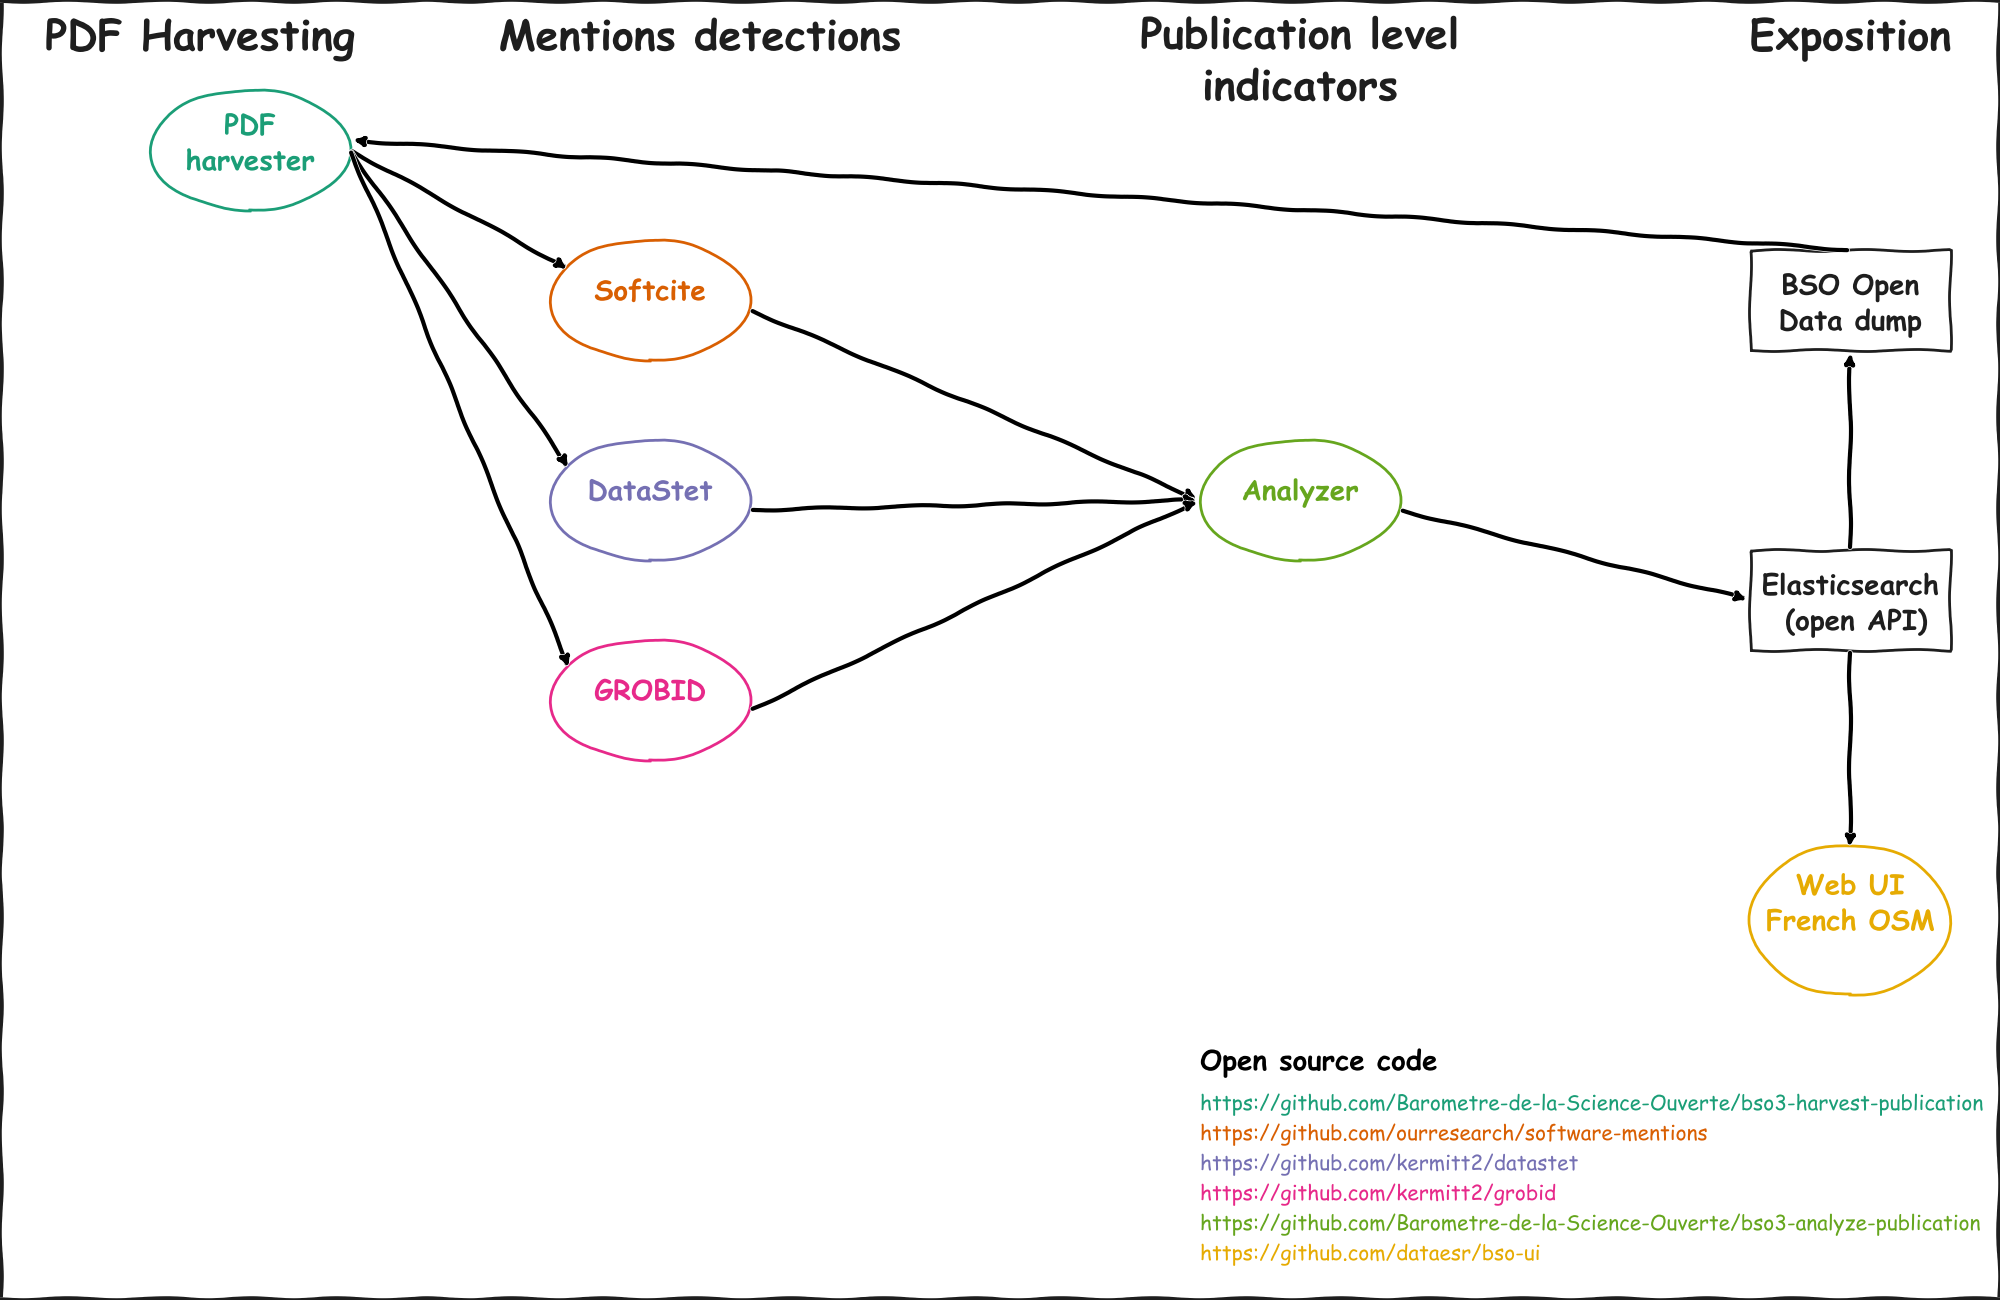
\includegraphics[width=6.25in,height=\textheight]{https://raw.githubusercontent.com/Barometre-de-la-Science-Ouverte/bso3-techdoc/master/methodology/flow_chart_publications_bso3.png}
\caption{Global overview of the publications data flows}
\end{figure}

Workflow description

Infrastructure and runtime indications

\hypertarget{results}{%
\section{4. Results}\label{results}}

\hypertarget{full-text-harvesting}{%
\subsection{4.1 Full text harvesting}\label{full-text-harvesting}}

\begin{longtable}[]{@{}lcrr@{}}
\toprule
is\_oa & number of publications & number of PDF downloaded & \% download
success\tabularnewline
\midrule
\endhead
True & 698,610 & 616,733 & 88 \%\tabularnewline
False & 659,584 & 272,070 & 41 \%\tabularnewline
Total & 1,358,194 & 888,803 & 65 \%\tabularnewline
\bottomrule
\end{longtable}

\begin{longtable}[]{@{}lcr@{}}
\toprule
harvester\_type & number of PDF downloaded & \% of total\tabularnewline
\midrule
\endhead
standard & 559,332 & 63 \%\tabularnewline
Elsevier TDM API & 200,155 & 22 \%\tabularnewline
arXiv & 78,078 & 9 \%\tabularnewline
Wiley TDM API & 51,238 & 6 \%\tabularnewline
\bottomrule
\end{longtable}

\hypertarget{dataset-and-software-mention-extraction}{%
\subsection{4.2 Dataset and software mention
extraction}\label{dataset-and-software-mention-extraction}}

\hypertarget{research-product-deduplication}{%
\subsection{4.3 Research product
deduplication}\label{research-product-deduplication}}

\hypertarget{french-open-science-monitor-indicators-and-dashboards}{%
\subsection{4.4 French Open Science Monitor indicators and
dashboards}\label{french-open-science-monitor-indicators-and-dashboards}}

\ldots{}

One of the ojectives of the French Open Science Monitor is to provide
all research institutions with a local version of the indicators.
Similarly as for measuring the openness of research publications on the
existing platform, the new indicators can be bounded to datasets and
software produced by the researchers only affiliated to a particular
organization. The ability to measure the research activity at different
scale, from a given organization to the national level has led to the
creation of a BSO user group
(https://groupes.renater.fr/sympa/info/bso-etablissements).

\hypertarget{limitations-and-future-work}{%
\subsection{5 Limitations and future
work}\label{limitations-and-future-work}}

\hypertarget{limitations}{%
\subsubsection{5.1 Limitations}\label{limitations}}

\hypertarget{future-work}{%
\subsubsection{5.2 Future work}\label{future-work}}

\hypertarget{domain-coverage}{%
\paragraph{5.2.1 Domain coverage}\label{domain-coverage}}

\hypertarget{large-scale-research-entity-disambiguation}{%
\paragraph{5.2.2 Large-scale research entity
disambiguation}\label{large-scale-research-entity-disambiguation}}

\hypertarget{local-open-science-monitor}{%
\paragraph{5.2.3 Local Open Science
Monitor}\label{local-open-science-monitor}}

\hypertarget{data-and-software-availability}{%
\section{Data and software
availability}\label{data-and-software-availability}}

The data resulting from this work are publicly available on the French
Ministry of Higher Education, Research and Innovation open data portal:

The source code used for the French Open Science Monitor is available on
GitHub, and shared with open source licences.

\hypertarget{acknowledgements}{%
\section{Acknowledgements}\label{acknowledgements}}

Thank you to the readers.

\hypertarget{references}{%
\section*{References}\label{references}}
\addcontentsline{toc}{section}{References}

\hypertarget{refs}{}
\begin{cslreferences}
\leavevmode\hypertarget{ref-bracco_extending_2022}{}%
{[}1{]} Bracco, L. et al. 2022. Extending the open monitoring of open
science: A new framework for the French Open Science Monitor (BSO).
(2022).

\leavevmode\hypertarget{ref-du_softcite_2021}{}%
{[}2{]} Du, C. et al. 2021. Softcite dataset: A dataset of software
mentions in biomedical and economic research publications. \emph{Journal
of the Association for Information Science and Technology}. 72, 7 (Jul.
2021), 870--884. DOI:\url{https://doi.org/10.1002/asi.24454}.

\leavevmode\hypertarget{ref-mesri_2nd_2021}{}%
{[}3{]} MESRI 2021. 2nd National Plan for Open Science.

\leavevmode\hypertarget{ref-mesri_national_2018}{}%
{[}4{]} MESRI 2018. National Plan for Open Science.
\end{cslreferences}


\end{document}
